%%==================================================
%% chapter02.tex for SJTU Master Thesis
%% based on CASthesis
%% modified by wei.jianwen@gmail.com
%% Encoding: UTF-8
%%==================================================
% \bibliography{../bib/chap1,../bib/chap2}
\chapter{Hessian-Affine兴趣点检测算法}
\label{chap:algorithm}
  本算法可以在图像经过仿射变换或者尺度变换后寻找到相应的兴趣点,为了完成这样的目标,本算法基于如下理论\cite{mikolajczyk2004scale}:
  \begin{itemize}
    \item 通过Hessian矩阵检测出的兴趣点可以抵抗仿射变换的干扰,对相同的几何图案产生类似的响应;
    \item 尺度空间理论;
    \item 通过二阶矩量矩阵估测一个像素和哪些临近像素可以构成一个仿射形状。
  \end{itemize}
  本算法的主体流程如下\cite{Perdoch-CVPR-2009}:
  \begin{enumerate}
    \item 通过尺度空间理论构建不同的尺度空间;
    \item 在不同的尺度空间中,对每个3*3的像素块计算Hessian矩阵的响应,并找出在相邻尺度空间中响应最大的点;
    \item 计算这些点的仿射形状,如果存在仿射形状,将其均一化后计算SIFT描述符。
  \end{enumerate}
  通过这三步,可以排除尺度与镜头角度的影响,将图像中的关键点找出来。
  \section{尺度空间理论}
    由于计算机无法确定一个图像中物体的尺度,也就是说无从知道物体的大小,一个100像素的块可能是一片树叶也可能是一颗树;对于机器视觉系统,需要生成多个尺度空间,来抵抗尺度的干扰。尺度空间可以处理n维函数(计算机视觉中为2维),将其嵌入到一族单参数函数族中。这个单参数函数族就叫做尺度空间。为了生成多个尺度,通过多次降采样与高斯模糊来模拟人眼的特性。
    \subsection{高斯模糊}
      模糊算法可以认为是每个像素取周边像素的平均值,但是模糊算法需要一个核函数来决定怎样进行模糊运算。常用的模糊算法有均值模糊、高斯模糊、镜头模糊等,对应不同的核函数。
      \begin{figure}[!htp]
        \centering
        \subfigure[原图]{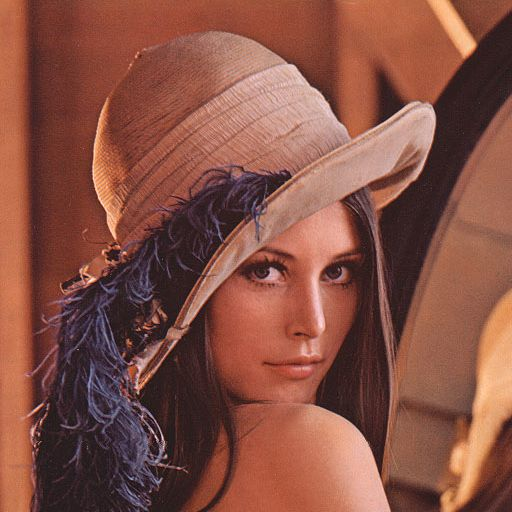
\includegraphics[width=0.2\textwidth]{chap2/lena}}
        \hspace{1cm}
        \subfigure[高斯模糊]{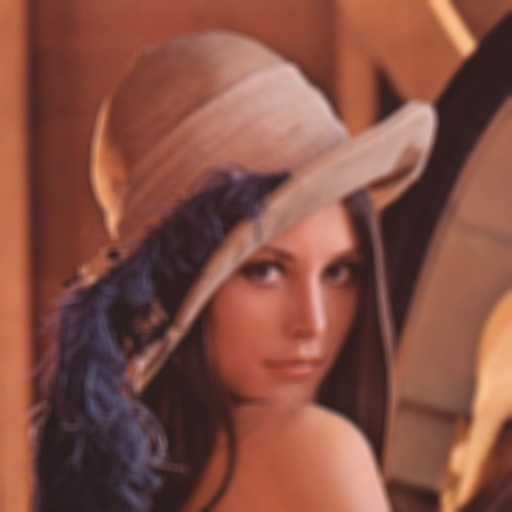
\includegraphics[width=0.2\textwidth]{chap2/lenaGauBlur}}
        \hspace{1cm}
        \subfigure[均值模糊]{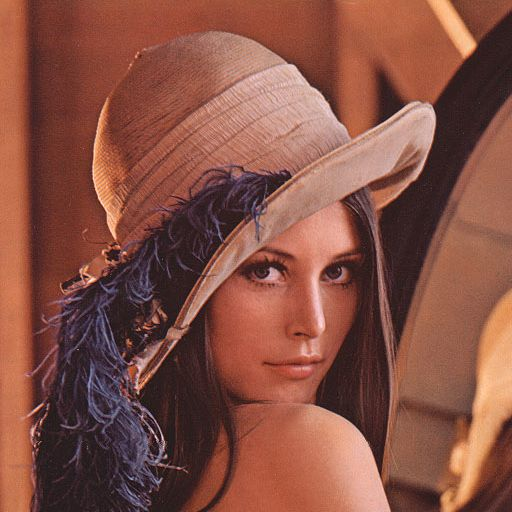
\includegraphics[width=0.2\textwidth]{chap2/lenaAvgBlur}}
        \caption{模糊算法示例}
      \end{figure}
      在本算法中,由于高斯函数满足如下尺度空间公理\cite{burt1983laplacian}:
      \begin{itemize}
        \item 线性
        \item 平移不变性
        \item 半群特性:$g(x,y,t_1)*g(x,y,t_2)=g(x,y,t_1+t_2)$
        \item 旋转不变性
        \item 正则性
      \end{itemize}
      这使得高斯卷积核是实现尺度变换的唯一线性核,因为高斯核对图像模糊不会引入其他噪声,高斯模糊使用正态分布作为核函数对图像进行卷积。正态分布的密度函数叫做高斯函数,在一维上表示为:
      \begin{equation}
        f(x,\sigma)=\frac{1}{\sigma\sqrt{2\pi}}e^{-x^{2}/2\sigma^2}
      \end{equation}
      将其推导到二维函数后:
      \begin{equation}
        G(x,y,\sigma)=\frac{1}{2\pi\sigma^2}e^{-(x^2+y^2)/2\sigma^2}
      \end{equation}
      则一副二维图像的尺度空间定义为:
      \begin{equation}
        L(x,y,\sigma)=G(x,y,\sigma)*I(x,y)
      \end{equation}
      其中$\sigma$是尺度,决定了图像的平滑程度,尺度越大细节越少,$(x,y)$是图片的空间坐标。在本算法中,对一个分辨率下的图片使用不同的尺度$\sigma$进行高斯模糊,初始的尺度$initialSigma$与尺度空间数量$numberOfScales$可以通过代码进行控制。
      \begin{figure}[htp]
        \centering
        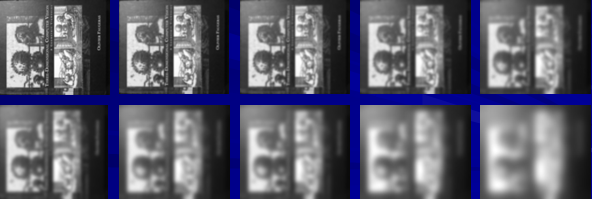
\includegraphics[width=0.7\textwidth]{chap2/multiSigma}
        \caption{高斯模糊中,不同$\sigma$下的一张图片}
      \end{figure}
    \subsection{高斯金字塔}
      为了构建高斯金字塔,一般需要如下几个步骤\cite{sivic2005discovering}:首先,图像经过一个低通滤波器进行平滑(本算法使用高斯模糊),然后,对这个平滑后的图像进行抽样(一般抽样比例在水平和竖直方向上都为1/2),从而得到一系列的缩小的图像。对于高斯金字塔,很容易直观地理解为对同一尺寸的图像,然后进行不同程度的高斯平滑,这些图像构成高斯金字塔,这种是不对的,这描述的图像集合叫做一个八度。金字塔总要有个变“尖”的过程,真正的高斯金字塔要有个平滑以及下采样的过程,因此整个图像平滑以及下采样再平滑,构成的所有图像集合才构成了图像的高斯金字塔。
      \begin{figure}[htp]
        \centering
        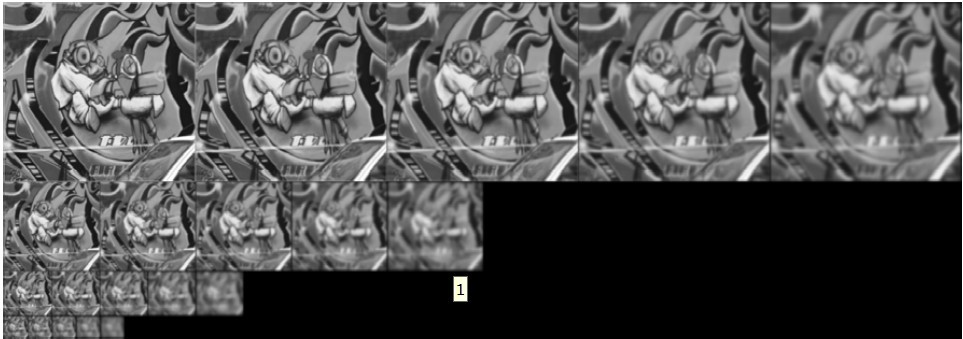
\includegraphics[width=0.7\textwidth]{chap2/multiOctave}
        \caption{不同尺度空间下的一张图片}
      \end{figure}
      \begin{wrapfigure}{r}{0.25\textwidth}
        \centering
        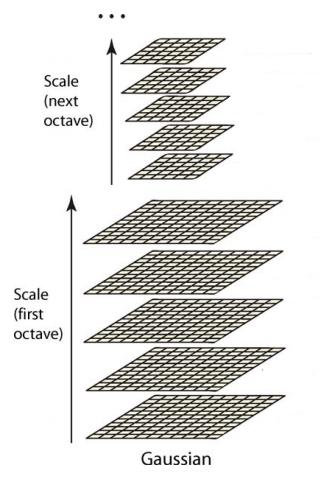
\includegraphics[width=0.2\textwidth]{chap2/pyramid}
        \caption{金字塔}
      \end{wrapfigure}
      高斯金字塔构建过程中,一般首先将图像扩大一倍,在扩大的图像的基础之上构建高斯金字塔,然后对该尺寸下图像进行高斯模糊,几幅模糊之后的图像集合构成了一个八度,然后对该八度下的最模糊的一幅图像进行下采样的过程,长和宽分别缩短一倍,图像面积变为原来四分之一。
      这幅图像就是下一个八度的初始图像,在初始图像图像的基础上完成属于这个八度的高斯模糊处理,以此类推完成整个算法所需要的所有八度构建,这样这个高斯金字塔就构建出来了。
  \section{Hessian响应}
    Hessian矩阵是一个自变量为向量的实值函数的二阶偏导组成的方矩阵,若函数如下:
    \begin{equation}
      f(x_1,x_2,\ldots,x_n)
    \end{equation}
    则它的Hessian矩阵为:
    \begin{equation}
    \begin{cases}
      H(f)_{ij}(x) & =D_iD_jf(x), x =(x_1,x_2,\ldots,x_n) \\
      H(f) & =\left[\begin{array}{cccc}
      \frac{\partial^2f}{\partial x_1^2} & \frac{\partial^2f}{\partial x_1 \partial x_2} & \cdots & \frac{\partial^2f}{\partial x_1 \partial x_n} \\
      \frac{\partial^2f}{\partial x_2 \partial x_1} & \frac{\partial^2f}{\partial x_2^2} & \cdots & \frac{\partial^2f}{\partial x_2 \partial x_n} \\
      \vdots & \vdots & \ddots & \vdots \\
      \frac{\partial^2f}{\partial x_n \partial x_1} & \frac{\partial^2f}{\partial x_n \partial x_2} & \cdots & \frac{\partial^2f}{\partial x_n^2} \\
      \end{array}\right] \\
    \end{cases}
    \end{equation}
    对于给定二阶导数连续的函数$f:\mathbb{R}^2\Rightarrow\mathbb{R}$,Hessian矩阵的行列式可以用于分辨$f$的临界点是鞍点或者是极值点。
    \begin{equation}
      H=\left|\begin{array}{cc}
      \frac{\partial^2f}{\partial x^2} & \frac{\partial^2f}{\partial x\partial y} \\
      \frac{\partial^2f}{\partial x\partial y} & \frac{\partial^2f}{\partial y^2} \\
      \end{array}\right|
      =\frac{\partial^2f}{\partial x^2}\frac{\partial^2f}{\partial y^2}-(\frac{\partial^2f}{\partial x \partial y})^2
    \end{equation}
    若$H>0$,则$(x,y)$是局部最大点或者局部最小点;若$H=0$,则$(x,y)$是鞍点。
    \subsection{粗略寻找特征点} 
      算法计算不同尺度中每个点的Hessian响应,也就是说在一个采样率下的不同尺度中,计算出Hessian响应并构建金字塔。由于金字塔是一个三维空间(平面图像二维,尺度一维),因此在三维空间中在寻找极大值点和极小值点。具体方法是比较当前特征点的值和其他26个点的值的\begin{wrapfigure}{r}{0.35\textwidth}
        \centering
        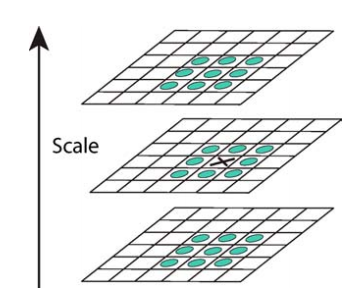
\includegraphics[width=0.3\textwidth]{chap2/localizePoints}
        \caption{寻找特征点}
      \end{wrapfigure}大小,这26个点包括:当前尺度下该点的8邻域以及前一尺度和后一尺度下与该点最近的9个点(9*2+8=26)。如果这个点是极大值或者极小值,则将其确定为待选点。
    \subsection{确定特征点位置}
      由于图像处于离散空间中,坐标都是整数,但是极值点的坐标不一定是整数,因此需要寻找到极值点的确定位置。对于一个自变量为离散量的函数,可以通过泰勒级数展开来拟合函数。由于每个点都在三维的空间当中,我们在尺度$\sigma$中的图像$D(x,y)$检测到了一个局部极值点,空间位置为$(x,y,\sigma)$,由于这是个离散极值点,在连续情况下极值点可能落在$(x,y,\sigma)$附近,其偏离$(x,y,\sigma)$的坐标为$(\Delta x,\Delta y,\Delta\sigma)$,对于$D(\Delta x,\Delta y,\Delta\sigma)$可以表示为在点$(x,y,\sigma)$的泰勒展开:
      \begin{equation}
      \begin{aligned}
        D(\Delta x,\Delta y,\Delta\sigma)=D(x,y,\sigma)+\left[
        \begin{array}{ccc}
          \frac{\partial D}{x} & \frac{\partial D}{y} & \frac{\partial D}{\sigma} \\
        \end{array}\right]\left[
        \begin{array}{c}
          \Delta x \\
          \Delta y \\
          \Delta \sigma \\
        \end{array}\right] \\
        +\frac{1}{2}\left[\begin{array}{ccc}
          \Delta x & \Delta y & \Delta\sigma \\
        \end{array}\right]
        \left[\begin{array}{ccc}
          \frac{\partial^2D}{\partial x^2} & \frac{\partial^2D}{\partial x\partial y} & \frac{\partial^2D}{\partial x\partial\sigma} \\
          \frac{\partial^2D}{\partial y\partial x} & \frac{\partial^2D}{\partial y^2} & \frac{\partial^2D}{\partial y\partial\sigma} \\
          \frac{\partial^2D}{\partial\sigma\partial x} & \frac{\partial^2D}{\partial \sigma\partial y} & \frac{\partial^2D}{\partial \sigma^2} \\
        \end{array}\right]
        \left[\begin{array}{c}
          \Delta x \\
          \Delta y \\
          \Delta \sigma \\
        \end{array}\right]
      \end{aligned}
      \end{equation}
      写成向量形式后:
      \begin{equation}
        D(x)=D+\frac{\partial D^T}{\partial x}\Delta x+\frac{1}{2}\Delta x^T\frac{\partial^2D^T}{\partial x^2}\Delta x
      \end{equation}
      最终可以算出:
      \begin{equation}
        \frac{\partial^2D}{\partial x^2}\Delta x=-\frac{\partial D(x)}{\partial x}
      \end{equation}
      如果得出其中一个向量的偏移大于0.6,则移动到相邻点上。通过最多5次的迭代,可以得到一个最终候选点的精确位置与尺度$\hat{x}$。
    \subsection{去除边缘点}
      由于Hessian矩阵对边缘点敏感,但边缘点对一些噪声不稳定\cite{ericsson2003affine},因此需要去除这些边缘点。Hessian矩阵的特征值$\alpha$与$\beta$有如下公式:
      \begin{equation}
        Tr(H)=D_{xx}+D_{yy}=\alpha+\beta
      \end{equation}
      \begin{equation}
        Det(H)=D_{xx}+D_{yy}-\left(D_{xy}\right)^2=\alpha\beta
      \end{equation}
      边缘点的特征为:跨越边缘的方向有较大的主曲率,与边缘相切的方向主曲率较小。因此,可以通过$\frac{\alpha}{\beta}$的比率函数并确定阈值来体现表征那些不好的边缘点,$\frac{\alpha}{\beta}$越大,说明这个点就越糟糕。设$r=\frac{\alpha}{\beta}$:
      \begin{equation}
        \label{equ:edgeEval}
        \frac{Tr(H)^2}{Det(H)}=\frac{\left(\alpha+\beta\right)^2}{\alpha\beta}=\frac{\left(r\beta+\beta\right)^2}{r\beta^2}=\frac{\left(r+1\right)^2}{r}
      \end{equation}
      由于\ref{equ:edgeEval}是关于$r$的增函数,所以可以通过这个公式判断$r$的大小,从而判断这个点是不是边缘点。
  \section{寻找标准仿射形状}
    由于图像可能经过仿射变换,为了找到一个兴趣点附近图形的标准仿射形状,引入了第二矩量矩阵\cite{ericsson2003affine,Perdoch-CVPR-2009,mikolajczyk2004scale,mikolajczyk2002affine,chiu2006matching}:
    \begin{equation*}
      M=\sum_{x,y}w(x,y)\left[\begin{array}{cc}
      I_x^2 & I_xI_y \\
      I_xI_y & I_y^2 \\
      \end{array}\right]
    \end{equation*}
    其中$w(x,y)$是窗口函数,本算法中使用高斯窗口,$I_{xy}$为函数在$(x,y)$时在$xy$方向的梯度。由于矩阵$M$是角对称阵,则其可以表示为:
    \begin{equation}
      M=R^{-1}\left[\begin{array}{cc}
      \lambda_1 & 0 \\
      0 & \lambda_2 \\
      \end{array}\right]R
    \end{equation}
    这个矩阵的特点是,如果图像经过仿射变换或者旋转变换,矩阵可以表示为$M_t=M_a^{-1}M_r^{-1}M_oM_rM_a$,其中$M_t$是经过变换后图形的第二矩量矩阵,$M_o$是变化前的第二矩量矩阵。这两个矩阵的特征向量相同。并且由于这个矩阵的表示类似于椭圆的表示:
    \begin{equation*}
    \left[\begin{array}{cc}
    u & v \\
    \end{array}\right]M
    \left[\begin{array}{c}
    u \\
    v \\
    \end{array}\right]
    \end{equation*}
    \begin{wrapfigure}{r}{0.45\textwidth}
      \centering
      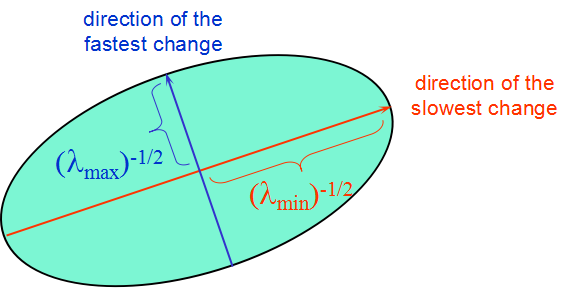
\includegraphics[width=0.4\textwidth]{chap2/ellipse}
      \caption{第二矩量矩阵的椭圆表示}
    \end{wrapfigure}
    所以将特征向量$\lambda_1$与$\lambda_2$看作是椭圆的长轴与短轴,矩阵$R$决定了椭圆的方向。算法首先将矩阵$R$设置为单位阵,$\lambda_1$与$\lambda_2$设置为1,这假定图形的响应是一个单位圆。随后通过插值将仿射图形映射到图片当中,生成一个19*19的计算窗口,然后计算这个窗口的第二矩量矩阵,并计算这个矩阵的平方根与特征值。通过特征值我们可以知道这个图形的相应距离单位圆还差多少。通过最多16次迭代,算法可以得到一个接近于单位圆的响应。
    \par
    在此之后,算法将均一化这个图形,对正主方向,并将其输出到19*19的块中,计算这个图形的SIFT描述符。到这里,整个算法就完成了,这个算法读取一张图片,计算Hessian响应,在有高相应的地方,寻找仿射形状并计算它们的SIFT描述符。


% https://hal.inria.fr/inria-00548252/document
% http://lis.csail.mit.edu/pubs/tlp/Matching-ICPR06.pdf
% http://www.robots.ox.ac.uk/~vgg/research/affine/det_eval_files/mikolajczyk_ijcv2004.pdf
% cpvr09b
% http://lear.inrialpes.fr/people/triggs/events/iccv03/cdrom/iccv03/1142_ericsson.pdf
